La presente distribuzione della materia risulta essere altamente disomogenea, organizzata in ampie strutture 
cosmiche, come i colossali ammassi (\textit{cluster}) di galassie tenuti insieme dalla
interazione gravitazionale tra i propri componenti, che raggiungono masse complessive tra $10^{13}$
e $10^{16}$ masse solari. Inoltre esistono sovrastrutture ancora più mastodontiche, dette superammassi.
I superammassi si presentano come un intricato reticolo di filamenti luminosi di galassie, che delimitano
spazi scuri, vuoti. La singolarità sottostante questo tipo di distribuzione è nota come \textit{caustica} e costituisce una 
patologia causata dalla trattazione fluida della materia, che ha invece natura discreta.
Strutture come quelle mostrate in Fig.\ref{fig:caustica} non sono presenti solo in cosmologia, ma 
si ritrovano in molteplici situazioni naturali. Per esempio, il nome caustica si riferisce anche alla scomposizione
della luce sul fondo di una piscina, che effettivamente forma un reticolo analogo alle distribuzioni galattiche.

\begin{center}
	\begin{figure}[H]
		\centering
		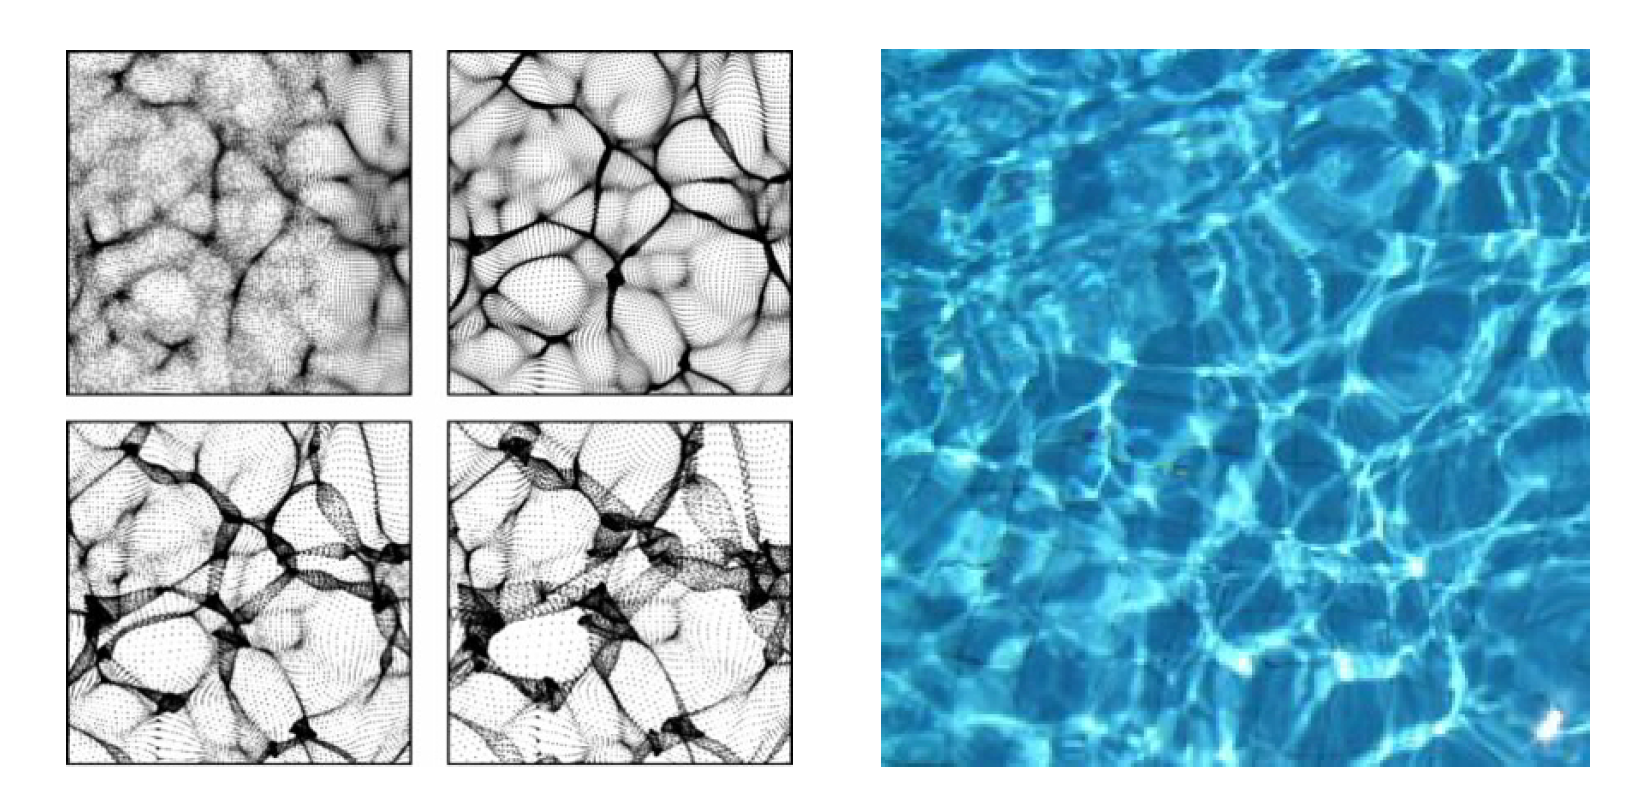
\includegraphics[scale=0.25, angle=0]{caustica.png}
        \caption{A sinistra, simulazione a N corpi bidimensionale fatta in approssimazione di Zel'dovich per crescenti
        oscillazioni di densità rispetto alla media $\rho_b$. A destra, caustica sul fondo di un piscina. Immagine tratta da \cite{gurbatov}.}
		\label{fig:caustica}
	\end{figure}
\end{center}
Questa distribuzione grumosa della massa si può descrivere con preciso approccio matematico, che sarà discusso nel primo capitolo,
e riguarda la teoria del \textit{trasporto ottimo}, che affronta il problema di determinare quel percorso massimamente
efficiente, ovvero con il minimo dispendio, attraverso cui si può trasportare una certa distribuzione di massa iniziale a una 
finale. La nascita delle teorie sul trasporto ottimo si deve a Gaspard Monge (1746-1818), che per primo formulò il principio
variazionale in senso statico. L'idea fu quella di scegliere una funzione costo e impostare la minimizzazione della stessa: 
per la formalizzazione matematica si può consultare la sezione (\ref{sec:metodi}). \'E interessante osservare che Monge 
arrivò a queste equazioni affrontando il problema di sterro e riporto, ossia quale fosse il metodo più efficace per scavare buche
e rinterrare il materiale altrove. Nel manuale di Cedric Villani (1973-presente) la stessa questione viene riformulata nei termini
di panetterie e café-bistrot: qual è il modo più efficiente per consegnare le brioches prodotte nei panifici a tutti i punti vendita,
note le densità di produzione e di consumo per ciascun punto? Come minimizzare i costi del trasporto?

Quasi due secoli dopo il problema fu ripreso da Leonid Kantorovich (1912-1986), premio Nobel per l'Economia nel 1975, nell'ambito 
dei suoi studi sulla Programmazione Lineare, teoria derivata dallo studio della pianificazione economica sovietica. Kantorovich si
rese conto solamente alcuni anni più tardi di avere generalizzato la discussione di Monge, scrivendone una versione generalizzata,
o rilassata, caratterizzata da imposizioni matematiche meno stringenti.

Le equazioni di Monge-Ampere-Kantorovich (MAK) trovano applicazione in una grande varietà di ambiti, in particolare è interessante 
soffermarsi sulla fisica matematica dei sistemi viventi \cite{cardin}. Il problema del trasporto del liquido ematico nei mammiferi,
finalizzato a trasportare il nutrimento secondo le necessità delle areee locali del corpo, è un problema di trasporto
ottimo che si può risolvere con MAK. Solitamente le densità di consumo locali sono note, pertanto è possibile impostare
il problema e spiegare in questo modo lo sviluppo della rete arteriosa, che è per natura disposta nel modo più efficiente.
Grazie all'impianto variazionale nel corso del Novecento si è quindi intavolato lo studio dei metabolismi animali.
Tuttavia le equazioni si prestano non solo alla descrizione dei meccanismi dell'alimentazione animale, ma anche al
mondo vegetale: è possibile infatti anche descrivere il regime di approvvigionamento di una pianta, o meglio 
la ramificazione delle sue radici nel sottosuolo.
Di recente un gruppo di matematici giapponesi (Tero, Kobayashi e Nakagaki) ha identificato un'applicazione nella
dinamica dell'evoluzione di una determinata specie di muffa unicellulare del fango (\textit{Physarium Polycephalum}),
guidata dalla via più efficiente per raggiungere fonti di alimentazione (\cite{yamada}).

\begin{center}
	\begin{figure}[H]
		\centering
		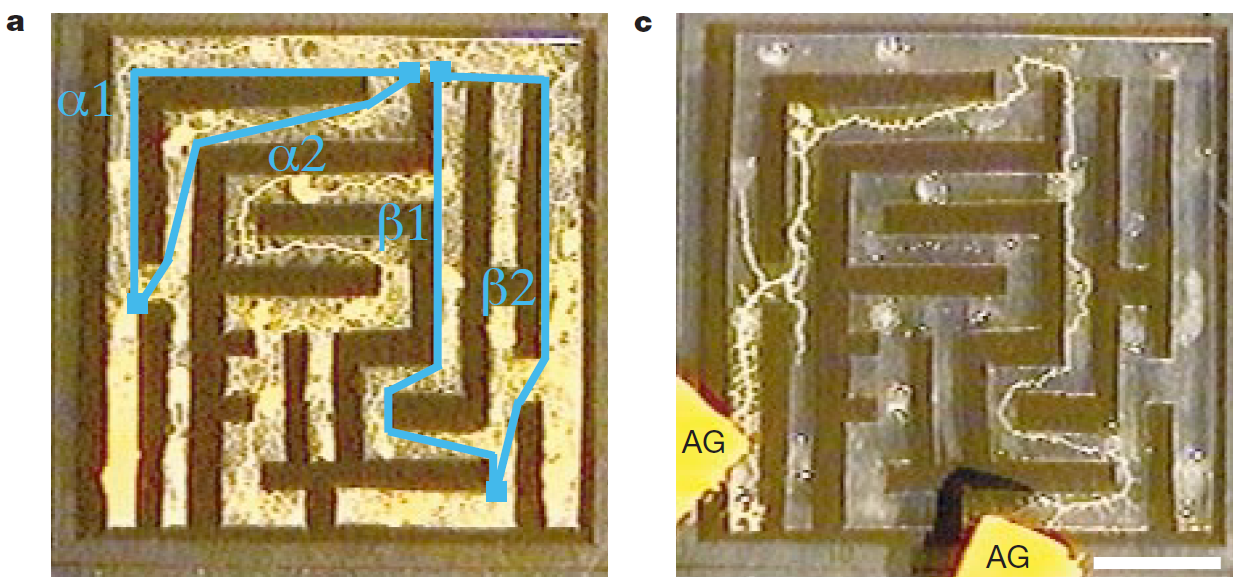
\includegraphics[scale=0.3, angle=0]{yamada.png}
		\caption{A sinistra sono raffigurati i possibili percorsi di sviluppo della muffa per raggiungere i fiocchi d'avena, inseriti all'interno 
		di un labirinto edificato su un piano di agar con pareti di pellicola di plastica. A destra	è schematizzata la situazione quattro ore dopo
		l'inserimento del cibo: è evidente che il fungo ha selezionato i due percorsi più brevi. Immagine tratta da \cite{yamada}.}
		\label{fig:yamada}
	\end{figure}
\end{center}
Lo straordinario comportamento della muffa mostra segni di primitiva intelligenza cellulare.

Tornando alla cosmologia, nella prima parte dell'elaborato saranno citate le equazioni MAK tra i metodi di ricostruzione della densità di materia
nell'universo, assieme ad altre tecniche. Nella seconda parte invece vedremo una trattazione fluida nel caso unidimensionale,
con conseguente formazione di caustiche, delle quali sarà fornita una classificazione.